\chapter{\sysname: A Low-Latency FaaS Research Control Plane}
\label{chap:iluvatar}

Providing efficient Functions as a Service (FaaS) is challenging due to the serverless programming model and highly heterogeneous and dynamic workloads. 
% Great strides have been made in optimizing FaaS performance through scheduling, caching, virtualization, and other resource management techniques.
% The combination of these advances and growing FaaS workloads have pushed the performance bottleneck into the control plane itself.
Current open-source FaaS control planes like OpenWhisk introduce 100s of milliseconds of latency overhead, and are becoming unsuitable for high performance FaaS research and deployments.
In this chapter we present the design and implementation of \sysname, a fast, modular, extensible FaaS control plane which reduces the latency overhead by more than two orders of magnitude.
\sysname~has a worker-centric architecture and introduces a new function queue technique for managing function scheduling and overcommitment. 
\sysname~is implemented in Rust in about 13,000 lines of code, and introduces only 3ms of latency overhead under a wide range of loads, which is more than 2 orders of magnitude lower than OpenWhisk. 


% \section{Why a new Serverless GPU Approach?}
\section{Challenges in providing GPU acceleration for Functions}
\label{sec:motiv}

The current resources offered by serverless platforms severely limit the types of function workloads it can support.
% They are limited to a few GB of memory and limited vCPU time~\cite{lambda-limits}.
Memory is limited to a few GB and vCPU access is restricted to a single, timesliced, core~\cite{lambda-limits}.
Yet any function with a dataset that exceeds these limits or a problem space that needs parallel computing for timely results cannot be served.
% Moving computation to a GPU by providing faster solutions and increased device memory that is much more than current serverless limits.
GPU acceleration alleviates both of these bottlenecks and has the double benefit of improving existing workloads. 
We can't get this acceleration without cost unfortunately, several considerations need to be made for their benefits to shine.

\begin{comment}
\begin{table}
  \caption{Cold starts with a GPU can be worse because of container startup and library initialization. 
  If the execution is significant, this delay can still be a minor part of the latency.
  All times are in seconds.}
  \begin{tabular}{lrrr}
    \hline
    Function & GPU & CPU & GPU Speedup \\
    \hline
  FFT & 3.322 & 13.073 & 3.94x \\
  Ffmpeg & 4.612 & 34.260 & 7.43x \\
  Imagenet & 11.286 & 10.103 & 0.9x \\
  Roberta & 15.481 & 14.372 & 0.93x \\
  Eos & 4.904 & 1.049 & 0.22x \\
  Isoneural & 9.963 & 1.434 & 0.15x \\
  Lavamd & 2.136 & 14.161 & 6.64x \\
  Lud & 2.359 & 110.495 & 46.85x \\
  Myocyte & 4.339 & 39.662 & 9.15x \\
  Needle & 2.177 & 223.306 & 102.58x \\
  Pathfinder & 1.797 & 106.667 & 59.37x \\
  Srad & 3.945 & 123.499 & 31.31x \\
  Squeezenet & 6.793 & 4.672 & 0.69x \\
  RNN & 2.491 & 3.226 & 1.3x \\
  \end{tabular}
\end{table}
\end{comment}

\begin{table}
  \caption{Attaching a GPU adds significant time to container startup overhead. All times are in seconds.}
  \label{tab:gpu-attatch}
  \vspace{\captionspace}
  \begin{tabular}{lccc}
    \hline
    Function & GPU & No-GPU & Cold-Start Slowdown \\
    \hline
  Imagenet & 8.581 & 6.907 & 1.25x \\
  Roberta & 16.374 & 14.015 & 1.17x \\
  % Squeezenet & 5.809 & 3.966 & 1.47x \\
  % RNN & 4.284 & 3.776 & 1.14x \\
  Ffmpeg & 2.044 & 0.775 & 2.64x \\
  FFT & 2.648 & 3.677 & 0.73x \\
  % Eos & 2.408 & 1.589 & 1.52x \\
  Isoneural & 2.586 & 1.662 & 1.56x \\
  % Lavamd & 1.947 & 1.223 & 1.6x \\
  Lud & 2.125 & 0.736 & 2.89x \\
  Myocyte & 2.145 & 0.980 & 2.19x \\
  Needle & 2.292 & 1.453 & 1.58x \\
  Pathfinder & 1.997 & 1.029 & 1.95x \\
  % Srad & 2.213 & 3.313 & 0.67x \\
  \end{tabular}
  \vspace{-0.4cm}
\end{table}

\subsection{GPUs Containers}

\begin{comment}
GPU resources are not a free upgrade and must be treated differently from classical FaaS resource management.
Memory on a single device is limited to 10s of GB of memory compared to potential TBs supported by their hosts.
% To make matters worse, unmodified applications can allocate the entire device's memory range, preventing other functions from running without deleting the current one.
To make matters worse, an unmodified application can allocate the entire device's memory range, leaving the control plane with no recourse but removal to relieve pressure.
We cannot limit compute usage of a GPU as easily as one can use cgroups to limit a process' vCPU time.
Device compute kernels are arbitrarily sized, and are not guaranteed to be constant across function inputs.
Reducing the size of kernel launches (i.e. the number of threads it executes on) will increase execution time for the application and may cause crashes.
Launching multiple concurrent kernels which exceed the device's capabilities results in throttling, negatively affecting user latency.
% Function execution and container management must therefore
Ensuring memory and compute are available for function execution, while avoiding container churn, are critical for usable performance.
% Applications also tend to be contstrained by one of these two resources, as has been shown repeatedly~\cite{}, making co-locating challenging.
We use UVM tricks and monitor GPU compute to accomplish both of these tasks, without having to control individual kernel launches that many other systems use~\cite{pemberton2022kernel,gu2023fast,ng2023paella}.
\end{comment}

Serverless invocations are run inside isolated sandboxes, and creation of these typically happens on the critical execution path.
Such \quotes{cold starts} add significant latency to an invocation in comparison to actual function execution time.
Runtimes for functions are on the order of tens of milliseconds~\cite{shahrad2020serverless}, yet container startup may be several seconds: an order magnitude delay.

Creating a new container with an attached GPU is even more expensive.
Table~\ref{tab:gpu-attatch} compares the startup time for new Docker containers with and without a GPU.
Cold start times grow up to 3x, {adding an average of 1.5 seconds of latency} to an already costly process~\cite{du2020catalyzer,lin_mitigating_2019,manner_cold_2018,mohan_agile_2019}.
% Creating a new container with an attached GPU is also costly, Table~\ref{tab:gpu-attatch} compares the startup time for new Docker containers with and without a GPU.
We captured and broke down time spent starting a new ML inference container with and without an attached GPU in Figure~\ref{fig:cold-timeline}.
The bottom timeline with attachment has an additional second of startup from an Nvidia library hook performing kernel work.
% , even before counting time taken by the application for initializing the GPU and loading specialized libraries.
% has the accelerator and spends roughly 1.5 seconds in an Nvidia library hook that performs kernel work to attach the GPU to the container.
Once that is accomplished, the control plane agent starts loading user function code, which uses a more complicated startup procedure to prepare the device and allocate resources, taking an additional 1.5 seconds.
All serverless platforms use a warm-start pool of containers to amortize the cold start penalties across future invocations.
We created first such container pool for avoiding GPU cold starts using our memory multiplexing and manipulation techniques.
% These seconds exacerbate existing cold start overheads already seen~\cite{du2020catalyzer,lin_mitigating_2019,manner_cold_2018,mohan_agile_2019}, which are often longer than function execution time.
% All serverless platforms use a warm-start pool of containers amortize cold start penalties across subsequent invocations which GPU limitations have precluded.
% Our techniques provide the first warm-start pool of GPU containers in serverless to significantly improve latency.
% Without the ability to share a GPU resources, specifically memory, between several containers, this 
% The combination of limited memory for containers, plus high overhead times

\begin{figure}
  \includegraphics[width=0.45\textwidth]{../graphs/coldstart/combined_timeline.pdf}
  \vspace*{-0.35cm}
  \caption{Time spent in a cold start without (top) and with (bottom) a GPU attached to a container hosting TensorFlow inference code.
          % Several additional seconds are caused by Nvidia runtimes and user code library loading.
          GPU attachment adds over a second to initialization time, 
          and user code setup of the GPU increases agent startup inside the container. 
          }
    \label{fig:cold-timeline}
% Gunicorn & library load time, no GPU:
% gunicorn: 0:00:11.688722
% Gunicorn & library load time, GPU:
% gunicorn: 0:00:13.320342
% nvidia: 0:00:01.399233
\vspace*{-0.6cm}
\end{figure}

\subsection{Serverless Scheduling}

% The workloads in FaaS are unique challenge in cloud computing, and make getting good performance out of GPU acceleration a complex challenge.
The workloads in FaaS are highly heterogeneous and represent a unique orchestration challenge in cloud computing.
Memory usage, execution duration, and the inter-arrival-time between invocations can vary by several orders of magnitude~\cite{shahrad2020serverless}.


Previous GPU-enabling works do not address the potential for worker-level queuing of accelerated Serverless functions.
The first proposal~\cite{naranjo2020accelerated} used Docker and only shows performance improvement against CPU runtimes, neither queuing nor any drawbacks from switching computation are considered. 
Several examples~\cite{pemberton2022kernel,gu2023fast,ng2023paella} do schedule ML inference tasks and GPU resources for high GPU utilization, but do so by breaking apart each function to control kernel launches, thereby preclude whole classes of applications from running.

% Existing platforms avoid queuing, and if at all implemented use a simple policy such as FCFS (first-come-first-serve). 
Most scheduling serverless work targets cluster load balancing via locality~\cite{faaslb-hpdc22,kaffes_hermod_2022,abdi2023palette,package-cristina-19}, and avoid queuing at workers.
% A naïve queuing algorithm such as FCFS (first-come-first-serve) or Round Robin works well with CPU scheduling because it can rely on a large pool of containers.
If necessary they use First-Come-First-Serve (FCFS), which works well scheduling on CPUs because it can rely on a large pool of containers to avoid cold starts and expects little queuing of invocations.
Unfortunately, a FCFS policy neither take into account the need for fairness between functions under queuing, nor optimal use of limited device resources.
Moving data between host and device to change the running application is slow, as seen by~\cite{yu2019automatic, hong2017gpu} and we show below in Section~\ref{sec:shim}.
A new scheduling policy that considers locality of data on device and locality of functions in a smaller container warm pool are needed for viable GPU performance.
% Our memory multiplexing and manipulation
% However, the challenge of GPU locality and warm-pool leads these to high rates of cold starts, container churn, and loss of fairness.

% GPU functions also need data to be local

% Maintaining locality has seen much work~\cite{faaslb-hpdc22,kaffes_hermod_2022,abdi2023palette}, all trying to handle the highly heterogeneous~\cite{shahrad2020serverless} workloads of FaaS.
% Inter-arrival-times for functions can vary by several orders of magnitude, as do runtime characteristics such as execution time and memory usage.
% Inter-arrival-times for functions can vary by several orders of magnitude and are not fixed, complicating predicting when and how many containers will be needed.

% The CPU-GPU architecture differences require analyzing how FaaS keeps latency low, and determining how GPUs can fit in.
% Large host memory footprints are taken advantage of by FaaS to run the many containers needed to maintain high locality unpredictable functions.
% Limited GPU memory diminishes the chance for a local container warm hit, highlighting the need for a sizable container pool.
% Recently run functions will also benefit from architecture features like cache presence, and subsequent runs are less likely to need to pull external data dependencies.
% The large number of CPU cores on servers increases invocation concurrency

% A similar correlation exists with GPUs, they run faster when their data is \quotes{local} (i.e. on-device), as we show in our experiments in Section~\ref{sec:shim}.
% We resolve both problems with one solution: oversubscribe device resources and manipulate it for better locality.

% The limited resources of GPUs need a more advanced scheduler to provide \emph{locality}
% Our queue design can run invocations out-of-order, allowing several dispatches of a function in succession to increase warm hits, lowering latency.

GPU batching has been effective~\cite{ali_batch_2020,yang2022infless,ali2022optimizing} in improving GPU utilization and latency when executing ML tasks.
The inputs of multiple invocations are merged into one \emph{batch} by the control plane, computed together, and split apart to distribute results.
% Scientific applications among others are not amenable to batching, and for those that do, they require changing the FaaS paradigm.
Such white-box solutions eschew isolation by making assumptions about the workload, the fact that inputs can be manipulated and how function code can make use of them.
Scientific applications among others are not amenable to batching as their inputs cannot be merged in an attempt at more efficient computation.
Black-box scheduling that works with all application classes is required for generic adoption of accelerators in cloud serverless platforms.


\subsection{Balancing Workloads}

% Serverless relies on \emph{locality} to achieve low latency, a warm container isn't the only factor in this.
% Enabling new worklaods to run on serverless platforms is not sufficient, the workflow must also be fast and unobtrusive. 
% Users expect good \emph{performance} out of the control plane, else they will host their application another way.
% Serverless relies on \emph{locality} to achieve its low latency target, having both a warm container and data be present on-device for optimal results.
% Finally, platforms must be \emph{fair} and prevent function starvation when sharing compute time.

To demonstrate that our system achieves fairness with high performance and locality, we run a trace from our experiments (Sec.~\ref{sec:queue-knobs}) and compare the CPU vs GPU performance.
This representative workload is run on two systems: one with 48 CPU cores, and the other with two Nvidia P100 GPUs.
The functions are restricted to only use one of the two compute types, and the outcome is in Figure~\ref{fig:cpu-compare}.
% The GPU system, despite having lower compute concurrency, has 50\% lower latency 
The GPU system cannot run as many functions concurrently, requiring queuing, but still achieves 50\% lower latency over its CPU-only counterpart.
% These are performance gains and application opportunities which are currently being left on the table by because of the lack of compute parallelism, and which we are the first to enable.

% GPUs have become pervasive as a way of accelerating computation of all types, and are common in cloud computing offerings.
% Yet outside research proposals, they have not been integrated into serverless computing platforms.

\begin{figure}
  \includegraphics[width=0.45\textwidth]{../graphs/cpu_compare/25.7/compute_compare_squish.pdf}
  \vspace*{\captionspace}
  \caption{Average invocation latency for a trace is 2x better on a small GPU platform running our desigin compared to a CPU-only system.}
    \label{fig:cpu-compare}
    \vspace{-0.6cm}
\end{figure}


\section{Design}

In this section, we describe the load-balancing algorithm which is locality, load, and burst aware.

\subsection{Design Criteria}
\begin{enumerate}
\item Locality aware 
\item Burst tolerance 
\item Doesnt require Consistent global state of containers
\item Tolerant to stale loads
\item Practical
\item Not fully centralized: Partially decentralized. Important for scaling since replies go through LB as well and has to keep track of a lot of state. 
\end{enumerate}

\subsection{High-level overview}
Derived from CH-BL, with its guarantees.


\subsection{Locality with Bounded Loads}

Forward functions on overflow to the next one in the ring.
Advantages over other methods. Locality is very important. So if we ``overflow'' a server, there is a higher chance of a keep-alive cache ``hit'' 

We combine bounded loads and consistent hashing into a \textbf{CH-BL} policy.
Starting with the function's hash chosen node, we loop around the ring looking for a server who's load is below the bounded ceiling.
The first matching server is sent the invocation. 
Algorithm~\ref{algo:BoundedLoadsPolicy}

\begin{figure}
  \begin{algorithmic}[1]
    \State $bounded\_ceil \gets 1.2$
    \For{$Server \gets ServerRing$}
      \State $L \gets Server.load$
      \If{$L \leq bounded\_ceil$}
        \State \textbf{Send to server Server}
      \EndIf
    \EndFor
    \State \textbf{Send to random server}
  \end{algorithmic}
  \caption{Bounded Loads Locality Policy}
\label{algo:BoundedLoadsPolicy}    
\end{figure}

\subsection{Caching Aware Forwarding}

% Impact of the warm starts is different for different functions. And so we use this information to make the forwarding decision. 
% FaasCache \cite{TODO} established not only that functions benifit from warm starts, but vary greatly between their cold and warm runtimes.
% It has been well established that functions benefit from being run warm, and that better cache eviction choices can improve warm hits.
Different functions can gain more from running warm than others, knowledge that is used in our FaasCache eviction strategy.
Our load balancer can then assume a function previously ran on a certain worker will still be warm unless under high load.
% If we mimic our eviction decision in our load balancing, we can better identify when locality has been trumped by high server load.   
% When the load  load balancer can rely on FaasCache locality keeping a function warm unless under very heavy loads. 
Unless the server's load is extremely high, we will gain benefit from the function running as a warm-hit, betting on locality, than a cold hit on a less loaded server.
We use the warm run speedup of $cold\_time / warm\_time$ as a load bound on our forwarding decision.
% The rule is ... \textbf{Derivation goes here}
This ratio can be extreme for some functions, with a warm time being an order of magnitude lower or more than the cold time, and must be curtailed to prevent skewed functions spamming their hashed server.
% Upper limit on this is currently 2.2 What's the justification? Linear slowdown limit? 
% Load of 1000 is clearly suboptimal. Plus need to think about the future as well. If it is bursty then we will probabilistically forward it anyways. So in the long run, better to spread it around.
To accomplish this we limit the \textit{slowdown} to some factor of \textit{bounded\_ceil} (typically 1-1.5) as seen in Algorithm~\ref{algo:ConsistentCachePolicy}.
We compute the predicted slowdown for the function's cold start and assign it to the first server on the ring whose load is less than the function's slowdown threshold.
% or expecting a warm hit on the server under quest 
% Thus the regret is a greedy regret and does not take into account future invocations. 


\begin{figure}
  \begin{algorithmic}[1]
    \State $slowdown \gets 1.2*(bounded\_ceil+1)$
    \If{$warm\_time \neq 0$}
      \State $r\_orig \gets cold\_time / warm\_time$
      \State $slowdown \gets min(r\_orig, slowdown)$
    \EndIf
    \State $thresh \gets slowdown-1.0$
    \For{$Server \gets ServerRing$}
      \State $L \gets Server.load$
      \If{$L - thresh \leq 0$}
        \State \textbf{Send to server Server}
      \EndIf
    \EndFor
    \State \textbf{Send to random server}
  \end{algorithmic}
  \caption{Default Consistent Caching Policy}
\label{algo:ConsistentCachePolicy}    
\end{figure}

\subsection{Handling Bursts}

Functions come in a variety of frequency classes and are also prone to unpredictable burstiness \cite{TODO}.
Identifying these bursts and both keeping latency for such "popular" functions low and preventing them from negatively impacting co-located functions is critical.
% Very popular functions can present problems.
We use two strategies:
1. Identify popular functions in a low-overhead online manner.
1a. Use this information to inform the load estimate. Due to the problem of \textbf{stale loads.}
2. Extreme overload: pick random server if going around the horn. 

\subsubsection{Popular function detection with Spatial Sampling}

Our solution to identifying popular functions and function bursts is inspired by SHARDS \cite{shards}.
We can identify the top \textit{p} percentile of functions, or filter on some IAT threshold, depending on what is desired. 
We use the former to avoid unnecessary hyperparamaters and, following SHARDS, randomly sampling invocations to track individual IATs.
This tracking is simplified by only recording the most recent access time, and then computing the IAT as an estimated moving average of the current IAT and  $now - last_access$.
These values are tracked for every function, and functions in the top $20^th$ percentile of IATs are considered \textbf{popular}.

\subsubsection{Load error correction}

Popular functions represent such a large percentage of invocations yet a small number of functions they can be safely spread across many servers without causing cold starts.
A fair load balancing algorithm \textbf{must} spread popular functions to ensure QoS for less frequent functions.
To achieve this, we introduce Gaussian noise to the forwarding decision.
% is added to the load based on the iat and the rate. Per-function noise. Can also be just a per-server estimate if desired. 
We compute the global arrival rate, then estimate the per-server arrival rate and the effect an invocation has on server load, following the steps in Algorithm~\ref{algo:PopularRLUPolicy}.
For each server we then sample noise from the normal distribution who's mean is centered on the \textit{anticip\_load}, and add that to the server's tracked load to get \textit{Lnoise}.
As with the previous policies, we iterate along the ring of servers until we find one who's \textit{Lnoise} is less than the global \textit{popular\_threshold}.

% \textbf{Question 1:} Why not do the stale load error correction for all functions, why just the popular ones?

\begin{figure}
  \begin{algorithmic}[1]
    \State $bounded\_ceil \gets 1.5$
    \State $arrival\_rate \gets 1.0 / avg\_iat$
    \State $server\_arrival\_rate \gets arrival\_rate / len(workers)$
    \State $anticip\_load \gets server\_arrival\_rate / worker\_cpus$
    \For{$Server \gets ServerRing$}
      \State $L \gets Server.load$
      \State $Lnoise \gets L + \mathcal{N}(\mu=anticip\_load,\,\sigma=0.1)$
      \If{$Lnoise \leq bounded\_ceil$}
        \State \textbf{Send to server Server}
      \EndIf
    \EndFor
    \State \textbf{Send to random server}
    \end{algorithmic}
\caption{Random Load Update Policy for popular functions}
\label{algo:PopularRLUPolicy}    
\end{figure}


\subsection{Putting it all together}

Unpopular functions still use Algorithm~\ref{algo:ConsistentCachePolicy}.
In all cases, if we exhaust the list of servers trying to find one with low load, we randomly assign the invocation to a server.
This only occurs in the most extreme cases of system load and also prevents spamming a popular server in that same scenario.



\section{Function Invocation Queuing}
\label{sec:q}

As a way to regulate and control function execution and worker load, \sysname~ incorporates a per-worker invocation queue architecture. 
Function invocations go through this queuing system before reaching the container manager, which either locates the warm container and runs the function or creates a new container.
Each worker manages its own queue, differentiating our design from OpenWhisk's shared Kafka queue. 

\noindent \textbf{Motivation.}
%
This queuing architecture is motivated by three main factors: i) the bursty nature of the workload , and ii) Reducing cold starts due to concurrent invocations, and iii) to give workers additional mechanisms for controlling their load, implementing prioritization, etc. 
Note that once the function passes through the queue, it is effectively ``scheduled'' for execution by the OS CPU scheduler.
The CPU scheduler of course has its own throttling and controling mechanisms, such as cgroups and the various scheduler tuning knobs.
The invocation queue thus acts as a kind of a regulator or a filter before the CPU scheduler, and ideally, ``feeds'' it the right functions at the right rates for maximizing throughput and minimizing latency.
%

Because function workloads are so bursty and heterogeneous, running each function immediately can significantly increase the worker load and result in severe resource contention and increase  function tail latencies.
%
The queue also helps as an explicit back-pressure mechanism for load-balancing, admission control, and elastic scaling.
The queue length is  used for accurately determining the true load on the worker, which is a vital input to consistent hashing with bounded loads~\cite{faaslb-hpdc22}.
This reduces the staleness and noise of using system load average as the load indicator, and makes load balancing more robust.


Queuing invocations also allows us to reduce cold starts.
While repeated function invocations are good and increase warm starts, 
\emph{concurrent} invocations of the same function results in cold starts for all the concurrent invocations, since each invocation needs to be run in its own container.
This is also the ``spawn start''~\cite{ristov_colder_warmer}, which causes severe latency increase of 10s of  seconds in public FaaS. 
If there are $n$ concurrent invocations that arrive at the same time, then the $n$ concurrent cold starts can significantly increase the system load and affect latency of other functions.
Instead, by queuing and throttling the functions, we can wait for the invocation to finish, and then use the warm container for the next function in this ``herd'', and so on and so forth. % Lol zizek 
%Having a queue allows us to regulate the invocations by this and other means. (?) 

% \vspace*{-8pt}
\subsection{Queue Architecture}
\label{sec:q:arch}

\sysname's queue architecture is shown in Figure~\ref{fig:arch}.
We have three main components.
%
From right to left, first, we have a concurrency regulator (or just regulator), which enforces the \textbf{concurrency limit}: the  upper-bound on the number of concurrently running functions. 
%
This lets functions execute ``on cpu'' without timesharing, and effectively determines the overcommitment ratio.
Higher concurrency limits (more than the number of CPUs) means  more CPU overcommitment.
Note that even with overcommitment, the cgroup quotas still provide proportional allocation (thus a 2 CPU container will still get twice the CPU cycles compared to a 1 CPU container). 
%
In addition to concurrency, other factors can also be used to regulate the queue discharge rate. 
The regulator can be used to run functions of only when sufficient resources (such as CPU bandwidth, warm containers, or even accelerators like GPUs) are available. 


%Note that technically the queue service backend is a processor sharing system, so can tolerate immediate execution albiet under heavy load.
%The concurrent cold start mitigation is one important component of the regulator policy.
%Its inputs are the number of currently running functions, the state of the container map to see which functions are executing, and the system resource utilization (load average, cpu\%, etc).
%This allows custom policies: we may want to limit the load average to under some limit, or the number of functions ``in flight'', etc.
\sysname~ can be deployed with a fixed concurrency limit based on the usage requirements, or use its dynamic concurrency limit mode. 
In the dynamic mode, we use a simple TCP-like AIMD~\cite{yang2000general} policy which increases the concurrency limit until we hit congestion, which in our case is hit if the system load average increases above some specified threshold. 
Other metrics are possible: looking at the increase in execution time (i.e., stretch) of the functions could also be used as a congestion metric.
The concurrency limit affects the tail-latency, and more advanced policies can be implemented. 


\begin{comment}
Having the container map also allows us to implement \textbf{concurrent cold start mitigation}.
If the function at the head of the queue has no warm containers available, and one of its instantiations is running, then we put the function back in the queue.
As a function's warm start is typically orders of magnitude shorter than cold starts, it is better for it to wait for warm container than to cold start one.
We implement this by asking the container pool for a warm container, and if it fails to give us one we can re-queue the invocation for the future.
Optionally, we can allow for a cold start to increase the number of warm containers for a function, naturally scaling if there is an increase in frequency.
\end{comment}

% This is currently implemented by looking at the container pool and estimating the likelihood of a warm vs. cold start, and using that expected execution time.
% The number of current concurrent executions are stored in the system statemap.


The second component is a \textbf{queuing discipline.} 
In the simplest case, we can use simple FCFS, and process functions in arrival order.
However, because functions are heterogeneous, this is not always the most appropriate.
Instead, we can use the past function execution characteristics such as their cold/warm running times for size-aware queuing such as shortest job first (SJF).
We elaborate more on the queuing policies in the next subsection. 

Finally, we note that queuing may increase the waiting time for small functions.
We thus have a \textbf{queue bypass} mechanism, which allows certain functions to bypass the queue and immediately and directly run on the CPU. 
Bypass policies take the function running time and the current system state as input. 
Currently, we implement a short-function bypass, where functions smaller than a certain duration are immediately scheduled, as long as the system is under a load-average limit.  
More effective bypass policies can also consider reinforcement learning approaches, since the action space is simple (bypass or enqueue), and the system state is well defined (functions running and in-queue, etc.).


% \vspace*{-8pt}
\subsection{Queuing Policies}
\label{sec:q:pol}

We implement multiple queue policies which leverage the repeated invocations of functions and use their learned execution characteristics to determining each function's priority.
To accomplish this, we maintain per-function characteristics such as cold time, warm time, and inter-arrival-time (IAT). 
%We maintain a sorted priority queue of invocations. 
We maintain a priority queue sorted by the function priorities, which are computed using their characteristics like arrival and execution time. 
%We can priority calculation to yeild differnt policy results.
%Different priority calculation yields different priorities. 

FIFO is simplest and invocations are just sorted by their arrival time.
For prioritizing small functions, we leverage our bypass mechanism, where the short functions can skip the queue and be scheduled directly on the CPU. 
Optimizing queuing policies for heterogeneous functions is challenging, and is an NP complete problem even in the offline case~\cite{bender1998flow}.


For improving throughput, we use shortest job first (SJF), which helps reduce the waiting time for short functions, but can lead to starvation for longer functions if the queue never drains. 
As a tradeoff between function duration and arrival, \sysname~ by default tries to minimize the ``effective deadline'' of a function, which is equal to the sum of its arrival time and (expected) execution time.
This earliest effective deadline first (EEDF) approach balances both short functions and starvation.
In both SJF and EEDF, an invocations' execution time is determined by its (moving window) warm time.
New/unseen functions have their times set to 0, to prioritize their execution.  
If we expect to find available containers for a function, we use its (moving window) warm time as the execution time in both SJF and EEDF.
Otherwise, we use its cold time---this also helps in reducing the concurrent cold starts, since the expected cold invocations of some functions in a burst separates them in the queue, and reduces the number of concurrently executing identical functions.
This spreading of function invocations over time increases the warm starts and overall performance. 
%
%Finally, we can  also prioritize functions with the highest inter-arrival-time. 
Finally, the RARE policy prioritizes the most unexpected functions (i.e., functions with the highest IAT). 

%All these policies can be combined with the short-function bypass technique.
%This also reduces the queue size and thus the overheads associated with maintaining a priority queue.
%In practice, the concurrency limit is larger than the number of the CPUs, so the queuing is expected to minimal under steady-state conditions. 


%L-p fairness:  $(\sum F^p)^{1/p}$


%%% Local Variables:
%%% mode: latex
%%% TeX-master: "paper"
%%% End:


\section{Implementation}
\label{sec:impl}

% Use a lot of provided stuff as a starting point
%   Containerd for isolation/container startup
%   CNI for networking
%   prebuilt Docker images
%   Rust language for efficient compiled language, without garbage collection interference
%   Tokio async handling & userspace threads

\sysname~is implemented in Rust in about 13,000 lines of code, and was made open-source and easy to use.
% It will be open-sourced upon paper acceptance. 
Its low latency and lack of jitter are attributable to the various low-level profile-guided performance optimizations we have implemented during the course of its development and testing.
Function handling and container management in the worker make up a majority of the implementation footprint and focus. 
Ours is a heavily asynchronous implementation using the \texttt{tokio} library in Rust, and various function lifecycle events spawn new userspace threads and trigger callbacks. 
The major data structure shared by the various worker threads is the container pool, which is implemented using the \texttt{dashmap} crate, which is a concurrent associative hashmap--- this provides noticeable latency improvements compared to a mutex or read-write lock.
Conversely, we still use a mutex for the queue, since we found minimal performance degradation compared to a no-queue architecture during profiling. 
These, and many other small optimizations, keep the \sysname~resource consumption small: even under a heavy and sustained load that saturates a 48 CPU server, the worker process uses less than 20\% of a single CPU core. 




%%%%%%%%%%%%%%%%%%%%%%%%%%%%%%

%\noindent \textbf{Agent Optimization.}
%All our functions are written Python, and we do some Python-specific optimizations during their prewarm.
%The agent imports the function Python code, loading it and any library dependencies into memory, plus executing statements not in functinos, such as downloading an ML model.


% \paragraph{Deployment}
% For ease of repeatable and scalable use, we have set up our system to be deployable with Ansible~\cite{}.
% In a command it can configure, set up, and tear down the applications that make up \sysname{}, and even capture artifacts like logs.
% It ties in nicely with the detailed configuration supported by our worker and controller services.
% Our services support configuration via a json file, convenient for development and local testing, but less so for large research experiments.
% Ansible, plus some clever config loading, allow us to inject arbitrary values as part of a larger command, making deployment for different experiments a breeze.

% With this setup, \sysname{} can be configured and deployed to any number of nodes with a single command.
% With this we easily scripted a variety of setups for our experiments in Section~\ref{Evaluation}, giving us consistent and controlled environments and results.
% Workers are configured with a json file on startup, with the various policy options (such as queuing), keep-alive, timeouts, networking, logging, etc.

% CNI and container-spec are also provided as json files. For the container-spec, we change....

% Workers have four main services: Containers, invocation, network, and status.

% \vspace*{-8pt}
\subsection{Support for FaaS research}
\label{sec:impl:support}

One of our major design goals is for a reliable and extensible control plane for performance-focused FaaS research.
We now describe some of the \sysname~features and our experiences in extending it.


\noindent \textbf{Performance Metrics.}
We keep track of all internal and external function metrics (such as their cold/warm execution time histories, inter arrival times, memory footprints, etc.) and provide them to all components of the control plane, and also to external services.
%
One of \sysname's implementation goals was to reduce the reliance on external services for system monitoring etc.
We thus track key system metrics like CPU usage, load averages, and even CPU performance counters and system energy usage using RAPL and external power meters.
These metrics are collected using async worker threads, and provide a single consistent view of the system performance.
%
Additionally, we also use and provide Rust-function tracing for fine-grained performance logging and analysis.
We use the \texttt{tracing} crate to instrument the passage of invocations through the control plane components, and obtain detailed function level timing information, which is used for identifying control plane and container-layer bottlenecks. 
%These logged details helped us with performance bottlenecks, but by default we keep disabled because it can increase per-invocation latency due to the overheads and CPU contention from creating so many logging events and it increases log file output size dramatically. 

\noindent \textbf{Adding New Policies and Backends.}
%
Using function and system metrics allows for easy development of data and statistical learning based resource management policies to be implemented.
Our baseline policy implementations for keep-alive eviction, queuing, load-balancing, are all easily extensible using Rust traits, polymorphism, and code generation. 
In our experience, adding new policies is relatively straight-forward, even for new-comers.
For example, all the priority-based queuing policies (SJF, EEDF, RARE, etc.) were implemented by extending the base FCFS policy.
Implementing and testing these policies took less than a few dozen lines and about four hours for a graduate student unfamiliar with the code-base. 

The default container runtime backend is \texttt{containerd}, but the interface is small, and supporting new backends is relatively easy.
We added Docker support in about 400 lines and one person-day of development effort.


\textbf{Load-generation and Testing.}
In the spirit of providing a full-featured system for FaaS experimentation, we have developed a load-generation framework.
It can do closed and open loop load generation, and be parameterized by the number and mixture of functions, their IAT distributions, etc. 
The testing framework can use functions from FaaS suites like FunctionBench~\cite{kim2019functionbench}, or custom sized functions that run lookbusy~\cite{lookbusy} for generating specific CPU and memory load.
%
The open-loop generation produces a timeseries of function invocations, which is helpful for repeatable experiments.
The functions' IAT distributions can be exponential, or be derived from empirical FaaS traces like the Azure trace~\cite{shahrad_serverless_2020}.


For the Azure trace, we start by randomly sampling functions and computing the CDF of their IATs.
We compute the expected load level in the system using Little's law, by finding the expected number of concurrent invocations for each function and adding them for all functions.
This expected load can be significantly different from the capabilities of the system under testing (for example, 100 concurrent functions will overload a 12 core system). 
Therefore, we can scale the individual function IAT CDFs to find a suitable load. This also allows us to change the relative popularities of individual functions, and conduct fine-grained sensitivity experimentation (like examining system performance when the popularity of one single function
changes, etc.).
We can generate larger traces by layering, and merging the traces from multiple smaller workloads.  


For synthetic functions (using lookbusy), we use their distribution of running times and memory consumption when generating the workload.
When using real functions from a benchmark-suite like FunctionBench, for each randomly sampled function, we use its average execution time (from the full trace), and assign it the closest function in the suite.
For example, if the average running time of a candidate function in the Azure trace is 8 seconds, we represent it using the ML-training function, which has the closest running time of 6 seconds.




%%%%%%%%%%%%%%%%%%%%%%%%%%%%%%


%%% Local Variables:
%%% mode: latex
%%% TeX-master: "paper"
%%% End:


\section{Experimental Evaluation}
\label{sec:ilu:eval}
We have extensively tested \sysname's performance characteristics throughout its development.
Here, we present a limited set of its key performance attributes and focus on new insights into FaaS performance.
All our experiments are conducted on a 48 core Intel Xeon platinum 8160 CPU, and we restrict the worker to 32 GB memory, running Ubuntu 20.04 using Rust version 1.67.0 and Tokio library version 1.19.2.
%
We are interested in evaluating latency overheads and \sysname's suitability as a low-jitter research control plane. 
This evaluation focuses exclusively on the performance of the worker, where we think most per-invocation latency improvement opportunities exist.
Many effective load-balancing policies have been published, but their impact on latency is limited to balancing decision time and warm start ratio.
Our stateless controller's overhead is consistent at less than 0.5ms, and we can thus ignore its latency contribution, for ease of exposition.
Our CH-BL based load-balancer maximizes locality and provides 99\% warm starts, and we focus on single-worker performance to remove unnecessary confounding factors.

% \noindent \textbf{Load Generation.}
% To collect benchmarking data and testing Control Plane Overhead for the different functions we generate \emph{closed loop} requests with varying client threads for 30 min each. We calculate the average for normalization of data collected in any other experiment. 

% For testing different Queue Policies we use open loop request generation. 

% \noindent \textbf{System Tweaks.}
% Ilúvatar itself keeps track of the memory usage and can limit number of concurrent requests dispatched to the system. We use Linux CPU Hotplug support to turn off some of the CPU cores to limit the system size. 

% \vspace*{-8pt}
\subsection{Control Plane and Function Performance}
\label{sec:ilu:eval:ovhead}

\begin{figure}
  \centering  \includegraphics[width=0.6\textwidth]{iluvatar/graphs/scaling/pyaes/overhead-scaling.pdf}
  \caption{The latency overhead of the control plane, as the number of concurrent invocations increases. 
        OpenWhisk overhead is significant and has high variance, resulting in high tail latency. 
        \sysname~reduces this overhead by 100x. }
  \label{fig:ow-scaling}
\end{figure}

\begin{comment}
\begin{figure}
    % Results for pyaes, which has runtime of ~300 ms
    % [0.8, 0.9, 0.99, 0.999, 0.9999, 0.9999]
    % 1 [2.26 2.29 2.40 4.40 4.59 4.59]
    % 2 [2.19 2.24 2.32 3.97 4.74 4.74]
    % 4 [2.28 2.32 3.07 4.81 5.76 5.76]
    % 8 [2.27 2.31 2.48 4.84 12.16 12.16]
    % 16 [2.60 3.02 4.65 7.89 8.66 8.66]
    % 32 [3.18 3.36 4.97 7.91 10.71 10.71]
    % 46 [5.02 6.19 14.50 20.25 26.02 26.02]
    % 48 [12.31 14.89 22.25 28.86 32.52 32.52]
  \includegraphics[width=0.6\textwidth]{iluvatar/graphs/scaling/pyaes/overhead-cdf.pdf}
    %  \vspace*{-6pt}
     \caption{\sysname~provides low latency overhead across a range of concurrent invocations.}
        % \vspace*{-6pt}
    \label{fig:ovh-cdf-aes}
\end{figure}
\end{comment}
% Results for lin_pack which has runtime of ~300 microseconds
% Percentiles: [0.8, 0.9, 0.99, 0.999, 0.9999, 0.9999]
% Thread count results (in milliseconds):
% 1 [2.69 3.01 5.68 940.41 956.48 956.48]
% 2 [2.69 2.94 7.12 940.17 942.17 942.17]
% 4 [2.16 2.53 5.74 928.90 935.37 935.37]
% 8 [2.00 2.35 4.78 833.26 860.58 860.58]
% 16 [3.13 3.70 7.05 664.69 709.56 709.56]
% 32 [6.30 7.54 13.78 351.35 430.77 430.77]
% 46 [9.62 11.83 20.14 103.92 15406.05 15406.05]
% 48 [9.64 12.14 20.85 73.48 31507.97 31507.97]

% Results for json_dumps_loads which has runtime of 0.5-1.5 seconds
% [0.8, 0.9, 0.99, 0.999, 0.9999, 0.9999]
% 1 [3.41 3.50 3.87 7.66 10.54 10.54]
% 2 [3.41 3.48 3.99 7.09 12.99 12.99]
% 4 [3.61 3.70 4.20 7.93 8.59 8.59]
% 8 [3.74 3.85 4.81 9.00 15.24 15.24]
% 16 [3.73 3.85 4.27 8.35 15.27 15.27]
% 32 [4.08 4.21 5.15 8.77 15.98 15.98]
% 46 [4.10 4.24 5.27 8.95 15.92 15.92]
% 48 [4.11 4.25 5.17 8.79 16.02 16.02]  

In this subsection, we focus on the latency overheads of \sysname~under different workloads and configurations.
For these experiments, we do not use any queuing, use a single worker, and focus on the most basic \sysname~configuration.  

We start by examining the control plane overheads under a closed-loop load for 30 minutes generated by different number of client threads. 
The control plane overhead CDF for the AES function is shown in Figure~\ref{fig:ow-scaling}. %~\ref{fig:ovh-cdf-aes} 
With 48 concurrent client threads, all the CPUs are fully utilized by function execution. 
Even in this saturated case, the 90 percentile overhead is less than 20ms. 
Just below this saturation limit, with 46 threads, the 90 percentile overhead drops to less than 10ms, and the average is less than 3ms. 

%%%%%%%%%%

\begin{figure*}
  \centering
  \subfloat[PyAES \label{fig:flow:pyaes}] {\includegraphics[width=0.3\textwidth]{iluvatar/graphs/scaling/pyaes/worker-e2e-and-exec.pdf}}
    \subfloat[JSON \label{fig:flow:json}] {\includegraphics[width=0.3\textwidth]{iluvatar/graphs/scaling/json_dumps_loads/worker-e2e-and-exec.pdf}}
    \subfloat[Video \label{fig:flow:video}] {\includegraphics[width=0.3\textwidth]{iluvatar/graphs/scaling/video_processing/worker-e2e-and-exec.pdf}}
      %  \vspace*{-6pt}
      \caption{End-to-end latency and execution times for different functions as we increase the concurrency levels.}
        %  \vspace*{-6pt}
  \label{fig:flow-fn-all}
\end{figure*}

We now provide a more detailed breakdown of the function latency.  
In Figure~\ref{fig:flow-fn-all}, we look at the end to end (E2E) function latency (i.e., flow time) and execution time of different representative functions under different loads.
The flow time is impacted by the control plane overhead and the function code execution time. 
Both these factors are affected by the system load, which in turn is affected by the concurrency level.
% We vary the number of clients invoking the same code in a closed loop, and had each client register the code as a unique function with the system.
The difference between the E2E and the function execution time is the control plane overhead, which is small for all functions and at all load levels.


Interestingly, a significant source of latency variance is the function execution time itself. 
For the small, CPU-intensive PyAES function (Figure~\ref{fig:flow:pyaes}), the  inter-quartile-range is 60ms, which is 20\% the average execution time.
Both the execution time (and hence the E2E latency) and the variance also increases with the system load.
%
This variance is also determined by the non-determinism in the function code.
For instance, the JSON function (Figure~\ref{fig:flow:json}) parses a random json file on every invocation, and thus has a higher natural variance in its execution time.
%
Finally, the video processing function is long and CPU intensive: it downloads and converts a video to grayscale. 
This magnifies the CPU contention, and the function latency increases from 6 to 9 seconds under heavy load.
%


The notable increase in execution time for all three functions is a result of  high  CPU cache miss percentage and a reduction in the instructions per cycle (IPC).
%
We also observed poor cache locality with an increasing number of CPU cores. When the same workload was run on half the number of CPUs (by disabling the rest of the CPU cores), the cache miss percentage significantly dropped (by more than 50\%), along with a proportionate reduction in the latency variance.
%
This highlights and emphasizes the deeper architectural challenges of FaaS, which were also shown by~\cite{shahrad_architectural_2019}. 
%We leave the study of the cause of this effect for future work.

\noindent \textbf{Result:} \emph{\sysname~overheads are small even under heavy load. Function code non-determinism and system load have a higher impact on the function execution times. }


%%%%%%%%%%%%%%%%%%%%

\begin{figure}
  \centering
  \includegraphics[width=0.6\textwidth]{iluvatar/graphs/impl/benchmark_cold_e2e.pdf}
  % \vspace*{-6pt}
  \caption{Most functions benefit from using a lower-level containerization and OS object caching on cold starts.}
  \label{fig:cold}
  % \vspace*{-6pt}  
\end{figure}

\noindent \textbf{Cold-starts.}
So far, we have focused on warm-start performance which dominates function workloads.
\sysname~also incorporates a few optimizations for cold-starts. 
Specifically, we are interested in quantifying the impact of the different container backends (containerd and Docker), and the network namespace caching optimizations. 
The end to end cold times for various functions are shown in Figure~\ref{fig:cold}: this includes both container startup time and function initialization overheads. 
In general, smaller functions face a larger impact due to the cold starts, since it represents a higher percentage of their total flow time. 


For small functions (left axis of the figure), using containerd (without network namespace caching) reduces the cold-start by more than 40\%, indicating a clear advantage of using a lighter container runtime.
Introducing the namespace caching further reduces the cold-start times by 15\% compared to unoptimized containerd which creates a new network namespace for each new container. 
After using the namespace cache, each function invocation sees upwards of $100 ms$ improvement in their cold start time.
%
The effects also hold for larger functions (right axis of Figure~\ref{fig:cold}), where Docker increases both the average and variance of the latency. 

% \vspace*{-8pt}
\subsection{Queuing Performance}
\label{sec:eval:q}

Having seen \sysname~performance in closed-loop micro-benchmarks, we now investigate the impact of its various queuing components and policies.
% We use our open-loop load-generation capabilities described in Section~\ref{sec:impl:support}.
We use an open-loop load-generator, with a random selection of 21 functions from the Azure traces, and pair them with different functions based on their closest running times.
This \quotes{stationary} workload has an average 40 requests per second for 30 minutes. 
This represents an extremely heterogeneous workload in terms of function durations and IATs.
Additionally, we also show results from a \quotes{bursty} workload generated in the same way, but with one function generating a burst of 18 requests per second for one minute.
In this open-loop testing, we prewarm the function containers to prevent excessive cold-starts immediately at the start of the workload.
The number of containers to prewarm for each function is determined using Little's law by using their average rates and execution times. 

%~\ref{tab:workload-dsc} lists selected functions and theirs IATs. To test effectiveness of the queue policies we modify the baseline trace to include a burst of function invocation at the rate of 18 request per second in the middle of baseline trace for a window of one minute. Application dd in the table~\ref{tab:workload-dsc} represents it's IAT in bold.
\begin{comment}
\begin{figure}
    \begin{tabular}{|c|c|l|l|}
        \hline
        Application        & \begin{tabular}[c]{@{}l@{}}Benchmark\\ E2E Time (s)\end{tabular} & \begin{tabular}[c]{@{}l@{}}Baseline\\ IATs (s)\end{tabular}                                                       & \begin{tabular}[c]{@{}l@{}}Burst\\ IATs (s)\end{tabular} \\ \hline
        chameleon          & 0.0138       & \begin{tabular}[c]{@{}l@{}}0.076, 0.212, \\ 0.263, 0.391, \\ 0.398, 0.993, \\ 1.527, 3.292, \\ 4.381\end{tabular} & \begin{tabular}[c]{@{}l@{}}0.076, 0.212, \\ 0.263, 0.391, \\ 0.398, 0.993, \\ 1.527, 3.292, \\ 4.381\end{tabular} \\ \hline
        dd                 & 0.105        & \begin{tabular}[c]{@{}l@{}}0.213, 0.501, \\ 5.255, 5.944\end{tabular}                                             & \begin{tabular}[c]{@{}l@{}}\textbf{0.0547}, 0.213, \\ 0.501, 5.255,\\ 5.944,\end{tabular}                                  \\ \hline
        gzip\_compression  & 0.222        & 5.984                                                                                                             & 5.984                                                                                                             \\ \hline
        json\_dumps\_loads & 0.420        & 0.499                                                                                                             & 0.499                                                                                                             \\ \hline
        image\_processing  & 1.969        & 4.043                                                                                                             & 4.043                                                                                                             \\ \hline
        model\_training    & 5.974        & \begin{tabular}[c]{@{}l@{}}2.445, 3.004, \\ 3.746, 5.982, \\ 6.045\end{tabular}                                   & \begin{tabular}[c]{@{}l@{}}2.445, 3.004, \\ 3.746, 5.982, \\ 6.045\end{tabular}                                   \\ \hline
    \end{tabular}%
    \caption{Description of Workloads used for evaluation.}
    \label{tab:workload-dsc}
\end{figure}
\end{comment}

\begin{figure*}
  \centering
  \subfloat[Overcommit \label{fig:q-base:wted}] {\includegraphics[width=0.5\textwidth]{iluvatar/graphs/old-baseline/breakdown/all_funcs_minheap_ed.pdf}}
  \hfill
  \subfloat[Distribution of function latencies \label{fig:q-base:box}] {\includegraphics[width=0.5\textwidth]{iluvatar/graphs/scaled_trace2/trace_0_1/violin_e2e_for_each_queue/16_16.pdf}}
  \hfill
  \subfloat[Latency breakdown \label{fig:q-base:breakdown}] {\includegraphics[width=0.5\textwidth]{iluvatar/graphs/scaled_trace2/trace_0_1/violin_func_breakdown/16_16.pdf}}
% \vspace*{-6pt}
  \caption{Queuing performance on the stationary Azure workload. Size-based policies can provide significant latency benefits.}
  \label{fig:q-baseline}
  %  \vspace*{-6pt}
\end{figure*}


\noindent \textbf{Metrics.} 
We use multiple performance metrics to understand and compare different policies.
Since functions can differ in execution time, we always normalize their total latency (flow time) by their execution time in an unloaded system. 
As shown in the previous figures~\ref{fig:flow-fn-all}, even with 1 closed-loop thread, the execution time has variance.
For normalization, we use the \emph{average} execution time with 1 thread for all the functions. 
Second, function popularities can also vary widely. 
We thus compute the \emph{weighted} latency, where each function's normalized latency is weighted by the number of its invocations in the trace.
Thus, the weighted latency represents the latency \emph{per-invocation}. 

\begin{figure}
  \centering 
  \includegraphics[width=0.6\textwidth]{iluvatar/graphs/scaling/WeakScaling.pdf}
    %  \vspace*{-6pt}
  \caption{The per-invocation function latencies for different system sizes (\# CPUs). We see a sharp inflection point at 16 CPUs, and use that in our queuing evaluation.}
    %  \vspace*{-6pt}
  \label{fig:weak}
\end{figure}


\noindent \textbf{Saturation Testing.}
We are primarily interested in how the queuing impacts the waiting time (which is part of the control plane overhead), and the function performance.
The analysis of queuing is interesting only in saturated scenarios, where there is enough extra load on the system and not all invocations can immediately run on the CPU.
We find this saturation point by weak scaling, and decreasing the number of CPU cores available to \sysname~(by disabling CPU cores using hot-unplug). 
The weighted and normalized latencies for different number of CPUs is shown in Figure~\ref{fig:weak}, which shows the performance \emph{without queuing.}
We see that for our baseline trace, increasing the number of available CPU cores has diminishing returns: the per-invocation latency doesnt benefit when CPUs are increased from 18 to 48.
However, we also see a sharp inflection point at 16 cores: decreasing the size to 14 cores results in a very high, almost $6\times$ slowdown. 
At 16 cores, our workload saturates the system, and we use this system configuration for all our queuing analysis.
We note that the alternative is to scale the workload up and run on on all 48 cores.
However, as we have shown previously through Figure~\ref{fig:flow-fn-all}, the poor hardware locality results in higher variance in the function execution times, and introduces more performance variance.
This variance often masks the control plane jitter, which is of more interest to us. 

% We evaluate our several queuing policies and compare them against a ``no-queue'' policy. 
% When there is no queue to limit concurrency, the control plane must either reject invocations when overloaded or allow resource overcommitment: namely processor sharing.
% Our system chooses the latter and will allow infinite invocations to run concurrently, so long as there is sufficient memory available, we do not overcommit memory.
% This behavior mimics how Openwhisk handles overload scenarios.
\begin{figure*}
  \centering
  \subfloat[Overcommit \label{fig:q-burst:wted}] {\includegraphics[width=0.5\textwidth]{iluvatar/graphs/scaled_burst_trace2/trace_0_1/barplot_breakdown_perqueue/all_funcs_minheap_ed.pdf}}
  \hfill
  \subfloat[Distribution of function latencies \label{fig:q-burst:box}] {\includegraphics[width=0.5\textwidth]{iluvatar/graphs/scaled_burst_trace2/trace_0_1/violin_e2e_for_each_queue/16_16.pdf}}
  \hfill
  \subfloat[Latency Breakdown \label{fig:q-burst:breakdown}] {\includegraphics[width=0.5\textwidth]{iluvatar/graphs/scaled_burst_trace2/trace_0_1/violin_func_breakdown/16_16.pdf}}
    %  \vspace*{-6pt}
  \caption{Small and bursty functions can get disproportionately impacted due to queuing. A little overcommitment can go a long way to reduce latency.}
    %  \vspace*{-6pt}
  \label{fig:q-burst}
\end{figure*}

\noindent \textbf{Impact of Overcommitment.}
Many frameworks like OpenWhisk inadvertently overcommit CPUs by running more functions than available CPU cores.
\sysname~can control the degree of overcommitment through its concurrency limit queue regulator.
Figure~\ref{fig:q-base:wted} shows the effect of this overcommitment, when the EEDF (earliest effective deadline) queue policy is used. 
The worker is limited to CPU cores, so higher concurrency limits represent different degrees of overcommitment. 
As the concurrency limit is increased, we see a reduction in the queuing time (which is a major part of the control plane overhead).
For instance, the queuing overhead is negligible when overcommitment level is 2 (i.e., 32 concurrency limit).
However we can see a tradeoff: the increased concurrency risks performance interference, and the code execution time also slightly increases (by 4\%).
For comparison and as a baseline, we also show the \quotes{no queue} configuration which is pure processor sharing and there is no limit on CPU overcommitment.
%
Queuing also reduces cold starts due to concurrent invocations. 
Without queuing, the number of cold-starts increased by more than $3\times$. 

For the bursty workload, the impact of overcommitment is even more drastic, as shown in Figure~\ref{fig:q-burst:wted}.
A slight increase in concurrency limit can reduce the weighted latency by more than $3\times$, indicating that overcommitment is more effective for burstier workloads.
Interestingly, the latency improves by $20\%$ with queuing as compared to the \quotes{infinite overcommitment} no queuing case.
This is due to the increase in function execution time due to uncontrolled CPU contention and interference, which the queue helps ameliorate. 

\noindent \textbf{Result:} \emph{CPU overcommitment can reduce queuing times, but come with risk of increased performance interference. \sysname's queue design provides a new effective \quotes{knob} for managing this tradeoff.}

% Bursty here. 

\noindent \textbf{Queuing Policies and Fairness.}
Next, we look at the performance impact of the different queuing policies themselves.
We are interested in the impact on the latencies of the different functions. 
Figure~\ref{fig:q-base:box} shows the normalized latencies of different functions with the different queuing policies.
This scenario has a significant amount of queuing: the concurrency limit is set to 16 (the number of CPUs). 
The function-size aware policies like SJF and EEDF provide much lower latency compared to the standard FCFS: the average latency is reduced by more than $2-3\times$. % 30 to 10 
%The RARE policy prioritizes the highest inter arrival time, and is not size aware, and also tends to suffer under high loads.

A breakdown of the latency of individual functions in Figure~\ref{fig:q-base:breakdown} helps understand this stark performance difference.
The queuing in FCFS increases the total time of the extremely small \quotes{web} function (13ms running time), which increases its latency by $30\times$.
The small-function prioritization by SJF and EEDF reduces this significantly. 

The impact of queuing for the bursty workload is even more interesting, as shown in Figure~\ref{fig:q-burst:box}.
EEDF's average latency is $2\times$ higher than simple FCFS, while SJF is 60\% lower than FCFS. 
Investigating the per-function breakdown again in Figure~\ref{fig:q-burst:breakdown} again points to the contribution of the small web function, which is \emph{also the bursty function}.
The bursty invocations trigger the cold-start mitigation, which deprioritizes them, and increases the queuing time, which disproportionately impacts the small functions.
% Bursty here. 

\noindent \textbf{Result:} \emph{Incorporating both function size and arrival times can improve function latency and fairness significantly. Very small functions see a higher \% increase due to queuing.}


%%%%%%%%%%%%%%%%%%%%%%%%%%%%%%


\noindent \textbf{\sysname~vs. Little's law vs. Simulation.}
Finally, we want to show \sysname's suitability for performance modeling, capacity planning, and as a research control plane for developing and evaluating FaaS resource management policies.
We compare the number of concurrent function invocations and queue length (EEDF) with the expected load according to Little's law, computed using average arrival rates and execution times of all functions of our stationary trace. 
We see that the real system metrics, even with all the inherent burstiness in the Azure trace, and the function execution and control plane jitter, are on average very close to the Little's law estimate.
This strongly indicates that our performance is indeed predictable even with highly heterogeneous workloads.

Additionally, Figure~\ref{fig:sim-vs-live-little} also shows the output of our ``simulation'' container backend described in Section~\ref{sec:design:ctr}.
This backend doesn't run actual function code, but exercises all other control plane aspects.
We use constant average function execution times (without accounting for variance and stochasticity) for all invocations.
Even though this simulation setup doesn't capture real-world variability and the impact of server load on function performance, we see that the simulation is also fairly closely aligned with the real experiment output.
This shows that \sysname's integrated simulation framework captures sufficient system dynamics and provides high-fidelity simulations.
This can significantly accelerate FaaS research, especially advances in reinforcement learning based scheduling, which requires high-quality simulations for learning policies. 

\begin{figure}
  \centering
  \includegraphics[width=0.6\textwidth]{iluvatar/graphs/trace-compare/baseline/minheap_ed/16/paper-status.pdf}
  \caption{\sysname~running in-silico closely models the in-situ performance. Making it a viable exploration opportunity supplementing real experiments.}
  \label{fig:sim-vs-live-little}
\end{figure}

% \subsection{Scalability}
% \label{sec:eval:scale}

% \textbf{Strong scaling. 48 worse than 16 because of ... bad locality?}

% \textbf{Simulation.}
% FaaS performance highly sensitive to workload due to skewed nature.
% Tough to experiment and report stable outcomes.
% For example, adding one function \emph{decreases} the overall latency. But its due to reporting.

% One way to avoid this is to look into simulations. Lightweight and allow different combinations to be thoroughly explored.

\begin{comment}
\noindent \textbf{Discussion.}
Our worker-centric design allows us to focus on single-worker performance. 
The load balancer is stateless and uses consistent hashing with bounded loads, and has a small overhead of less than 0.5 ms. 
Without workers sharing state (like with OpenWhisk's shared queue), there is no/minimal performance interference, and hotspots are confined in space and time.
%We conjecture that \sysname's performance improvements are largely due to the design and queuing policies for handling invocation bursts. 

Finally, our performance comparison with OpenWhisk is based on end-to-end latency testing. 
Performance tracing of OpenWhisk is challenging due to the highly distributed nature, and the drastically different architectures prevent a clean side-by-side comparison vs. the various components.
The use of Rust vs. Scala provides some performance gains as well, but all our OpenWhisk evaluation was conducted with ample heap sizes to reduce extra garbage collection overheads. 
\end{comment}

\begin{comment}
\begin{figure*}
  \centering
  \subfloat[Overcommit \label{fig:q-base:wted}] {\includegraphics[width=0.3\textwidth]{iluvatar/graphs/simulation/scaled_trace2/trace_0_1/barplot_breakdown_perqueue/all_funcs_minheap_ed.pdf}}
  \hfill
  \subfloat[Distribution of function latencies \label{fig:q-base:box}] {\includegraphics[width=0.3\textwidth]{iluvatar/graphs/simulation/scaled_trace2/trace_0_1/violin_e2e_for_each_queue/16_12.pdf}}
  \hfill
  \subfloat[Code Breakdown \label{fig:q-base:cold}] {\includegraphics[width=0.3\textwidth]{iluvatar/graphs/simulation/scaled_trace2/trace_0_1/violin_func_breakdown/16_12.pdf}}
 
  % \subfloat[Overcommit \label{fig:q-base:wted}] {\includegraphics[width=0.3\textwidth]{iluvatar/graphs/burst/breakdown/all_funcs_minheap_ed.pdf}}
  % \hfill
  % \subfloat[Fairness \label{fig:q-base:box}] {\includegraphics[width=0.3\textwidth]{iluvatar/graphs/burst/boxplot/16_24.pdf}}
  % \hfill
  % \subfloat[Cold \label{fig:q-base:cold}] {\includegraphics[width=0.3\textwidth]{iluvatar/graphs/burst/coldstarts/16_24.pdf}}
    % \vspace*{-6pt}
  \caption{Simulation baseline}
  \label{fig:q-burst}
    %  \vspace*{-6pt}
\end{figure*}
\end{comment}

%%% Local Variables:
%%% mode: latex
%%% TeX-master: "paper"
%%% End:


\section{Related Work}
\label{sec:related}

Alongside the closed-source FaaS control planes from the major cloud providers, a variety of other FaaS control planes exist.
Open-source production faas OpenWhisk~\cite{openwhisk}, OpenFaaS~\cite{openfaas}, nuclio~\cite{nuclio}, kNative~\cite{knative}, and funcX~\cite{funcx_hpdc_20}.
Others were made for with targeted research goals in mind \cite{jia2021nightcore, hendrickson2016serverless, oakes_sock_2018, singhvi2021atoll,vhive-asplos21}.

\sysname~ occupies a somewhat unique spot in the crowded FaaS landscape because of its focus on warm starts and some key constraints in our system design.
%
Techniques for reducing cold-start overheads, like snapshots, language isolation,  unikernels, all sit ``below'' the control plane, and can be complemented with fast control planes.
At the other extreme end, the predictable nature of serverless workloads has been used to great effect for predictive load-balancing, prefetching, sizing, etc.
\sysname~ is mostly reactive and is worker-centric, and tries to make minimal assumptions about workload predictability and focuses on more general optimizations that can work for arbitrary workload patterns.
%

\noindent \textbf{FaaS Control Planes.}
%
SOCK~\cite{oakes_sock_2018} is closely related to \sysname, and makes similar observations about network namespace overheads, and introduced storage and cgroup optimizations for serverless optimized containers. 
SOCK is based on OpenLambda~\cite{hendrickson2016serverless} and achieves great cold-start performance with Zygotes that are cloned into new containers.
These optimizations to the container runtime are also applicable to \sysname~ and are complementary. 
Using the standard containerd interface allows us to use multiple current and future container backends, and is a deliberate tradeoff. 
%Importantly it lacks both the ability to operate as a cluster and an integrated load generation system, both of which we have implemented both in \sysname~.


Nightcore~\cite{jia2021nightcore} is an integrated control plane and runtime system for low-latency microsecond-scale microservices.
It essentially implements containerized RPC, and uses fast message passing between the control plane and the agent.
Its special container runtime precludes generic ``black box'' functions, and it provides a weaker isolation model by running functions concurrently within the same container.
In the microservice context, container management and scheduling, dealing with heterogenenous functions, and other challenges are not relevant.


Atoll~\cite{singhvi2021atoll} is a fast and highly scalable control plane, and hugely benefits from pre-allocation and prediction.
It has a two level load-balancing setup with functions scheduled to a cluster group which then places them on a worker. 
\sysname's design and contributions are orthogonal to Atoll's more top-down and predictive approach, and we focus on the ``low-level'' worker problems.


Open-source control planes like OpenWhisk, OpenFaaS~\cite{openfaas}, nuclio~\cite{nuclio}, and kNative~\cite{knative}, are widely used to provide functions as a service. 
They tackle the competing demands of modularity and features, along with supporting function executions in generic environments.
Many FaaS systems use Kubernetes as the resource and container management layer, and its complexity and high latency further inhibits deep understanding and optimizations. 
OpenWhisk's cold and warm performance has been analyzed in many prior works such as~\cite{quevedo_evaluating_2019} and also as part of other systems~\cite{scheuner_lets_2022, alzayat_groundhog_2022, faaslb-hpdc22, faascache-asplos21}. 
OpenWhisk scheduling design and improvements can be found in ~\cite{kim_scheduling_2021, faaslb-hpdc22}.
Tighter latency requirements exist when deploying functions at the edge, and OpenWhisk's use on lower powered devices presents even more latency troubles~\cite{palade-edge-22, pfandzelter_tinyfaas_2020, hall_execution_2019, wang2021lass}. 
Interestingly, public cloud latencies are also significant, of the order of 50 ms~\cite{ustiugov_analyzing_2021}, hinting that the problems also extend their control planes. 
%All four of these control planes rely on Docker and Kubernetes for their deployment and scaling mechanisms.
%These existing tech stacks are highly useful, but limit the research possibilities of a platform, e.g. cold-start optimizations and deploying to edge nodes become intractable.
%While \sysname~ does have a Docker isolation implementation, it is to showcase the ability implement multiple containerization mechanisms and compare between them.


\noindent \textbf{Function Scheduling.}
Concurrent to our efforts, queuing of function invocations has been proposed in~\cite{zuk_call_2022}, which implements various size-aware policies like SJF. 
Surprisingly, and perhaps due to OpenWhisk overheads, their function slowdowns are extremely high: of more than $10,000\times$. 
An earlier theoretical queuing analysis of flow and stretch metrics is also presented in~\cite{zuk_scheduling_2020}. 
In contrast to \sysname's worker-centric design, a centralized core-level allocation design is presented in~\cite{kaffes_centralized_2019}.
In FaaS clusters, the tradeoffs in load balancing and early/late binding are evaluated in~\cite{kaffes_hermod_2022}.
Locality~\cite{faaslb-hpdc22}  and ML-based~\cite{yu2021faasrank} techniques for FaaS load-balancing take advantage of the high temporal locality and predictability of the FaaS workloads.
Our effort is more focused on reactive systems, and adding predictive allocation will only improve it. 

OS scheduler improvements can also improve FaaS workloads~\cite{fu2022sfs}. 
Regulating Linux CPU cgroups shares is also effective in overcommitment~\cite{ensure-faas-acsos20}.
Evaluating the effectiveness of these scheduling improvements when juxtaposed with queuing will be interesting. 
Scheduling function workflows and DAGs are a growing area~\cite{shen_defuse_2021,mahgoub_wisefuse_2022,zhou_qos-aware_2022}, and we focus on single-invocation optimizations. 

\begin{comment}
Restoring from snapshots~\cite{vhive, faasnap, catalyzer}


%The architectural implications are analyzed in~\cite{shahrad_architectural_2019}. We look at the higher levels of the stack, i.e., at the control plane. The paper identifies the fundamental factors affecting function performance at the hardware level due to cache misses, bad locality, etc. 
\paragraph{Edge.}
The lower resource availability of edge platforms also motivates lighter control planes. 
Tinyfaas is a apecialized FaaS platform for the edge 
\cite{pfandzelter_tinyfaas_2020}, but uses existing control planes like OpenWhisk and Kubless.
\cite{hall_execution_2019}


\paragraph{Scheduling.}

ANY papers that use previous running time/task size information!? Atoll. Aquatope. 

Tail latency: 50ms for warm-starts for the cloud. \cite{ustiugov_analyzing_2021} 

RL scheduling~\cite{yu2021faasrank}. 

Lets trace it\cite{scheuner_lets_2022} , platform overheads etc.


Workflow and serverless DAG scheduling is complementary to \sysname. 

FnSched. Anshul \cite{}. Centralized Scheduling? 

Sharing containers in SAND \cite{akkus_sand_2018}

Hierarchical scheduling (within container) in HyperFaas. 

\paragraph{OpenWhisk.}
\cite{quevedo_evaluating_2019} evaluates the cold and warm times under OpenWhisk. 
OW Hash based scheduling described in \cite{kim_scheduling_2021}.

Container sizing lot of attention, why! Uses OpenWhisk atleast\cite{guo_decomposing_2022}.
Also uses it and claims massive speedups. \cite{kotni2021faastlane}

Aquatope\cite{zhou_qos-aware_2022} also uses prewarming for keepalive and is based on OpenWhisk.

%%%%%%%%%

Overcommittment: Owl~\cite{tian_owl_2022} also does interference.
So does ENSURE and fnsched. Overcommittment has impact on both the function execution time and control plane overhead (more functions to execute and more contention of cplane processes with functions.) We do overcommitment for only short functions with the bypass. Longer functions likely to be CPU intensive.


Our work: control plane sandwiched between isolation optimizations and data-driven overcommit and predictive. 

Completely orthogonal to optimal sizing like sizeless~\cite{}, OFC~\cite{}, COSE~\cite{akhtar_cose_2020}, \cite{guo_decomposing_2022}, etc.
\end{comment}


\sysname~a fast, modular, and extensible FaaS control plane made open source capable of running on heterogeneous and edge hardware. 
It is implemented in Rust in about 13,000 lines of code, and introduces only 3ms of latency overhead under a wide range of loads.
Its worker-centric architecture, resource caching based design, queue-based overcommitment and scheduling, and careful asynchronous implementation, all contribute to low latency and jitter. 
% \sysname~is open source, runs on heterogeneous and edge hardware, and is intended to serve as a platform for future high-performance FaaS research and deployments.
% In the near future, we intend to incorporate support for Firecracker~\cite{firecracker-nsdi20} VMs and GPUs; investigate load balancing optimizations; and deploy \sysname~on HPC and cloud clusters. 
